\documentclass[a4paper,11pt]{article}
\usepackage[utf8]{inputenc}
\usepackage{amsmath, natbib, graphicx, enumerate, tikz, float, amsthm, verbatim, marvosym, physics, subfig}
\usepackage{hyperref}
\usetikzlibrary{patterns}
\usetikzlibrary{arrows.meta}
\usepackage[a4paper, total={7in, 10.5in}]{geometry}

\begin{document}

\title{Statistical Analysis II: Project 2 report}

\author{Kornel Howil}

\date{\today}

\maketitle

\section{Probabilities}
Knowing the bayesian network structure we can write that
\begin{equation}
    P(C|R,S,W) = P(C|R,S)\propto P(C, R, S) \propto P(C)P(S|C)P(R|C)
    \label{eq1}
\end{equation}
and
\begin{equation}
    P(R|C,S,W) \propto P(R,C,S,W) \propto P(C)P(S|C)P(R|C)P(W|R,S)
    \label{eq2}
\end{equation}
\subsection{$\mathbf{P(C=T|R=T, S=T, W=T)}$}
From equation \ref{eq1} we can write that
\[
    P(C=T|R=T, S=T, W=T) \propto 0.5 \cdot 0.1 \cdot 0.8 = 0.04
\]
and
\[
    P(C=F|R=T, S=T, W=T) \propto 0.5 \cdot 0.5 \cdot 0.2 = 0.05
\]
Hence after normalising
\[
    P(C=T|R=T, S=T, W=T) = \frac{0.04}{0.04 + 0.05} \approx 0.44
\]
\subsection{$\mathbf{P(C=T|R=F, S=T, W=T)}$}
From equation \ref{eq1} we can write that
\[
    P(C=T|R=F, S=T, W=T) \propto 0.5 \cdot 0.1 \cdot 0.2 = 0.01
\]
and
\[
    P(C=F|R=F, S=T, W=T) \propto 0.5 \cdot 0.5 \cdot 0.8 = 0.2
\]
Hence after normalising
\[
    P(C=T|R=T, S=T, W=T) = \frac{0.01}{0.01 + 0.2} \approx 0.05
\]
\subsection{$\mathbf{P(R=T|C=T, S=T, W=T)}$}
From equation \ref{eq2} we can write that
\[
    P(R=T|C=T, S=T, W=T) \propto 0.5 \cdot 0.1 \cdot 0.8 \cdot 0.99 = 0.0396
\]
and
\[
    P(R=F|C=T, S=T, W=T) \propto 0.5 \cdot 0.1 \cdot 0.2 \cdot 0.90 = 0.009
\]
Hence after normalising
\[
    P(R=T|C=T, S=T, W=T) = \frac{0.0396}{0.0396 + 0.009} \approx 0.81
\]
\subsection{$\mathbf{P(R=T|C=F, S=T, W=T)}$}
From equation \ref{eq2} we can write that
\[
    P(R=T|C=F, S=T, W=T) \propto 0.5 \cdot 0.5 \cdot 0.2 \cdot 0.99 = 0.0495
\]
and
\[
    P(R=F|C=F, S=T, W=T) \propto 0.5 \cdot 0.5 \cdot 0.8 \cdot 0.90 = 0.18
\]
Hence after normalising
\[
    P(R=T|C=F, S=T, W=T) = \frac{0.0495}{0.0495 + 0.18} \approx 0.22
\]
\section{Gibbs Sampler}
Using the calculated above probabilities, I implemented the Gibbs sampler in NumPy. This sampler was used to draw 100 samples 1000 times. This allowed us to make a histogram shown in the Figure \ref{fig1}.
\begin{figure}[H]
    \centering
    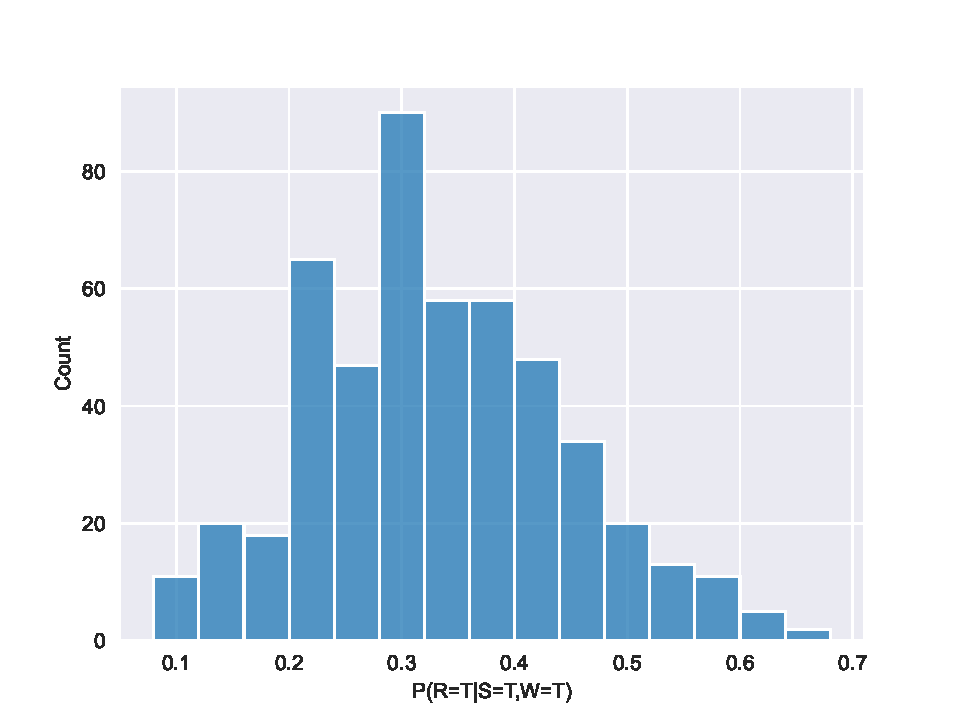
\includegraphics[scale = 0.86]{Plots/histogram100.pdf}
    \caption{Histogram of values of the conditional probability $P(R=T|S=T,W=T)$ obtained by sampling 100 values from Gibbs sampler 1000 times.}
    \label{fig1}
\end{figure}
\noindent Mean value of the probability is $ 0.3347$ and variance is equal to $0.0128$.
\section{Convergence diagnostics}
\subsection{Burn-in phase}
Gibbs sampler was used to sample 50000 samples 10 times. Relative frequencies were calculated for each of these 10 chains. Figures \ref{fig2} and \ref{fig3} show relative frequencies in the function of iteration all chains for respectively C=T and R=T.
\begin{figure}[H]
    \centering
    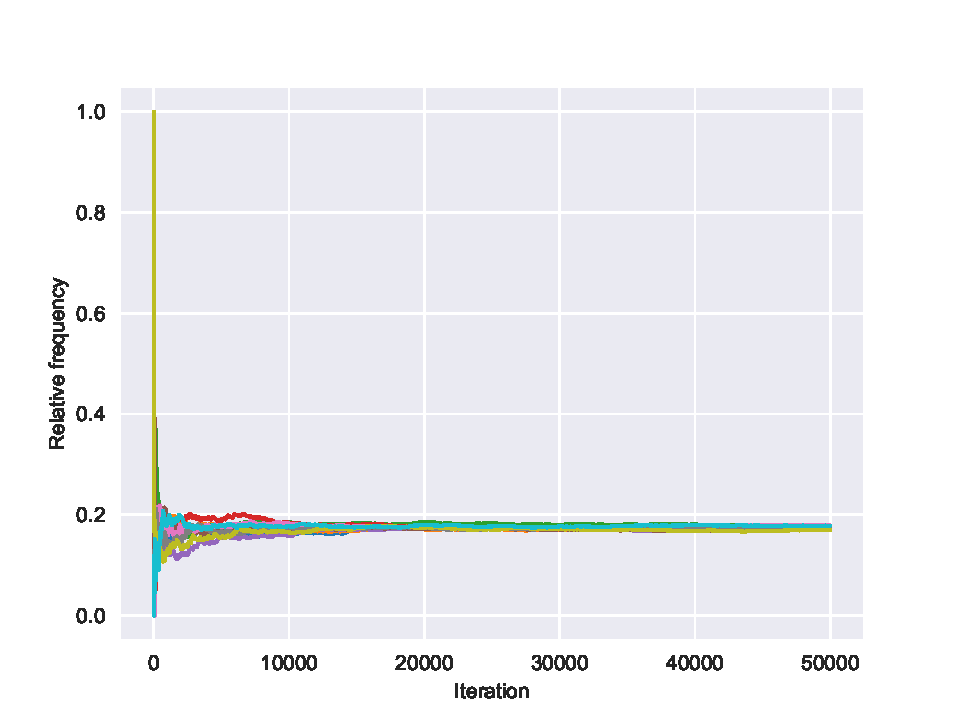
\includegraphics[scale = 0.86]{Plots/freqplot_cloudy.pdf}
    \caption{Relative frequencies in function of iteration of 10 chains for C=T.}
    \label{fig2}
\end{figure}
\begin{figure}[H]
    \centering
    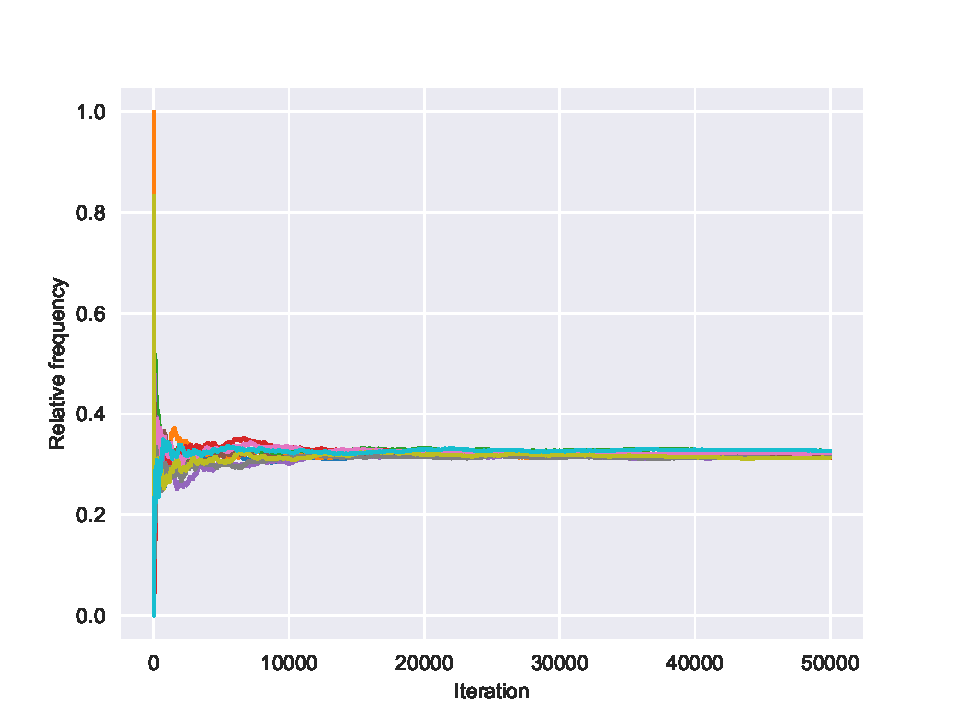
\includegraphics[scale = 0.86]{Plots/freqplot_rainy.pdf}
    \caption{Relative frequencies in function of iteration of 10 chains for R=T}
    \label{fig3}
\end{figure}
\noindent Using those plots we can estimate that burn-in phase lasting for 10000 iterations should be good enough.
\subsection{Autocorrelation}
Correlograms for both variables Cloud and Rain were produced using \texttt{plot\_acf} function from \texttt{statsmodels} package.
\begin{figure}[H]
    \centering
    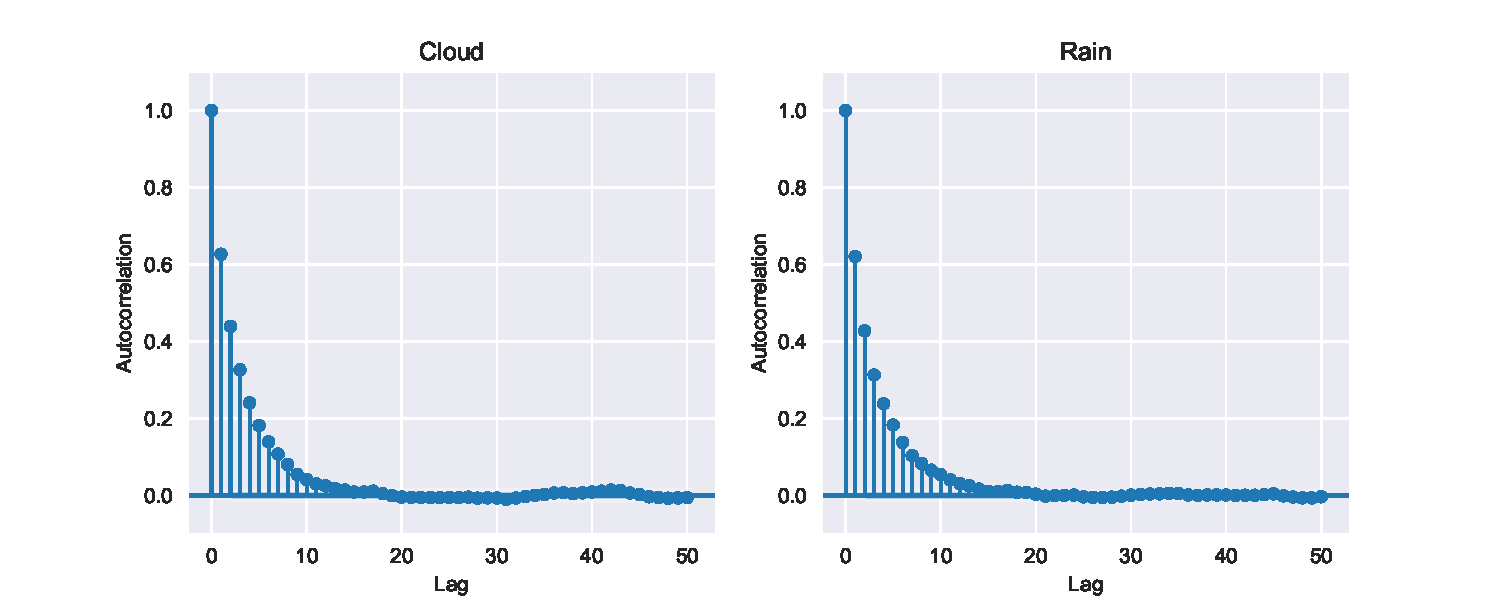
\includegraphics[scale = 0.7]{Plots/autocorrelation.pdf}
    \caption{Correlograms for both variables Cloud (left) and Rain (right).}
    \label{fig4}
\end{figure}
\noindent It can be seen from both figures that autocorrelation from lag greater than 15 is negligible. Hence, we can assume that keeping every 15-th sample would be  sufficient way to thin-out these chains.
\section{100 samples after burn\_in and thinning\_out}
Using chosen above values of burn\_in and thin\_out once again 100 samples (after burn\_in and thinning\_out) were drawn 500 times. Histogram of obtained conditional probabilities 
$P(R=T|S=T,W=T)$ is shown on the Figure \ref{fig5}.
\begin{figure}[H]
    \centering
    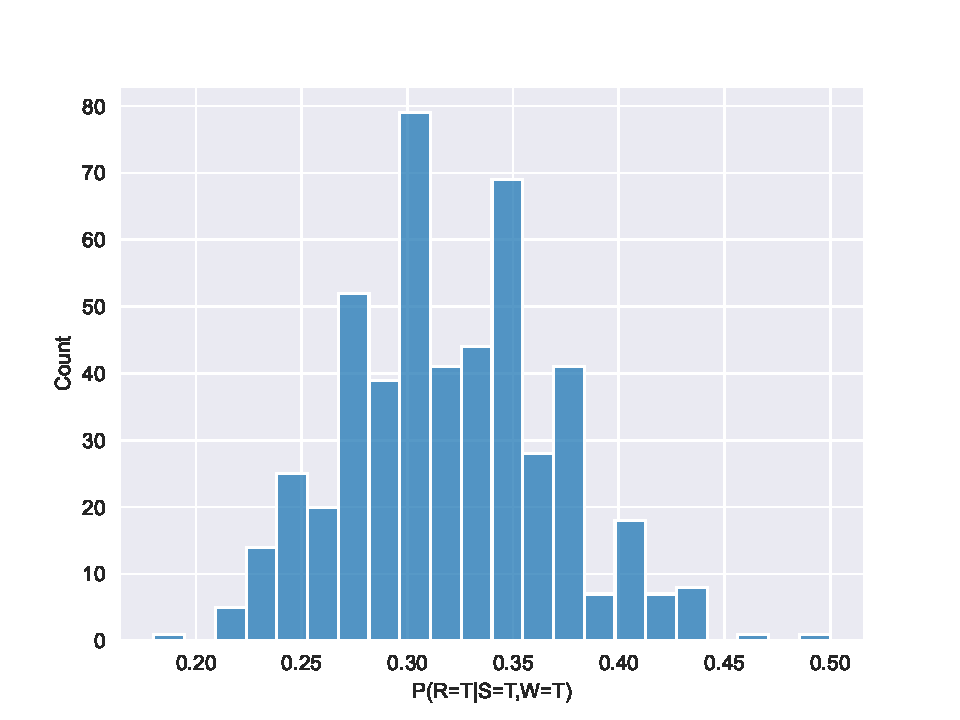
\includegraphics[scale = 0.86]{Plots/histogram100_bt.pdf}
    \caption{Histogram of values of the conditional probability $P(R=T|S=T,W=T)$ obtained by sampling 100 values (after burn\_in and thinning\_out) from Gibbs sampler 1000 times.}
    \label{fig5}
\end{figure}
\noindent The mean value of the conditional probability is 0.3196 and the variance is equal to 0.0024. We can see that variance is approximately 5 times smaller than in the run without burning\_in and thinning\_out. Hence, we can be more certain about the value of this probability.
\section{Final results}
\subsection{Final run of gibbs sampler}
For the final estimation of the $P(R=T|S=T,W=T)$ gibbs sampler was run 500 times for $n=50000$ iterations with chosen earlier values of burn\_in and thin\_out. Histogram of obtained conditional probabilities is shown on the Figure \ref{fig6}.
\begin{figure}[H]
    \centering
    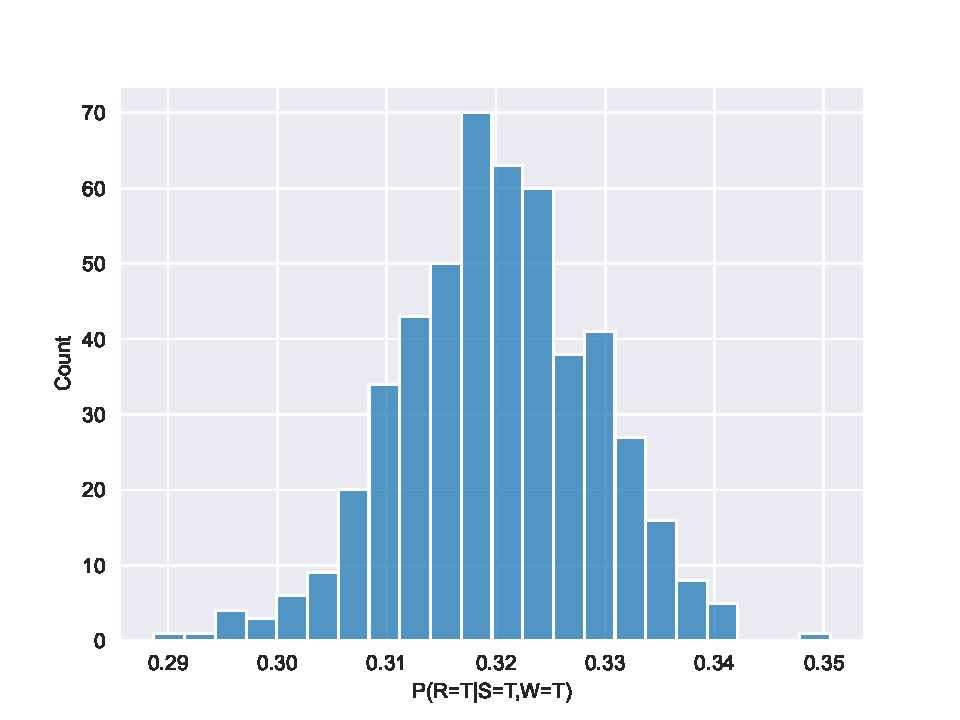
\includegraphics[scale = 0.85]{Plots/histogram50000.pdf}
    \caption{Histogram of values of the conditional probability $P(R=T|S=T,W=T)$ obtained by sampling 50000 values, burning\_in and thinning\_out from Gibbs sampler 1000 times.}
    \label{fig6}
\end{figure}
\noindent Mean value of the conditional probability is 0.3200 and variance is equal to $7.9845\cdot10^{-5}$. The variance is even smaller than in the last run with 100 samples.
\subsection{Exact result}
We can use values calculated in section 1 (before normalising) to calculate exact value of $P(R=T|S=T,W=T)$. Since
\[
    P(R=T|C=T,S=T,W=T) \propto 0.0396,
\]
\[
    P(R=F|C=T,S=T,W=T) \propto 0.0090,
\]
\[
    P(R=T|C=F,S=T,W=T) \propto 0.0495,
\]
\[
    P(R=F|C=F,S=T,W=T) \propto 0.1800,
\]
we can write that
\begin{equation}
    P(R=T|S=T,W=T) = \frac{0.0396 + 0.0495}{0.0396 + 0.0495 + 0.009 + 0.18} \approx 0.32039.
\end{equation}
In conclusion, result obtained from Gibbs sampler is very close to the exact value.
\section{Gelman-Rubin convergence test}
Gelman-Rubin convergence test was implemented according to the equation found in Vats and Knudson 2021  \cite{gr}.
\begin{equation}
    \hat{R} = \sqrt{\frac{\hat{\sigma}^2}{s^2}}.
\end{equation}
Convergence was tested on 100 samples without burning-in and thinning-out and 100 samples after both operations, with parameters found in section 3. Both times, the score was calculated based on $m=100$ chains. Results for samples without and with burning-in and thinning-out are shown respectively in \ref{w1} and \ref{w2}.
\begin{equation}
    \hat{R}_{\text{Cloud}} \approx 1.0341, \; \; \; \; \hat{R}_{\text{Rain}} \approx 1.0378
    \label{w1}
\end{equation}
\begin{equation}
    \hat{R}_{\text{Cloud}} \approx 1.0093, \; \; \; \; \hat{R}_{\text{Rain}} \approx 1.0095
    \label{w2}
\end{equation}
Assuming one of the most popular cutoffs of $\hat{R} < 1.01$ \cite{gr} we see that in the first case, the chains have not reached convergence and for the second case convergence has been reached.


\begin{thebibliography}{9}
\bibliographystyle{unsrt}
\bibitem{gr}
    Dootika Vats. Christina Knudson. "Revisiting the Gelman–Rubin Diagnostic." Statist. Sci. 36 (4) 518 - 529, November 2021. ,
    \emph{\href{https://doi.org/10.1214/20-STS812}{https://doi.org/10.1214/20-STS812}}

\end{thebibliography}
\end{document}